%%
%% GMU LaTeX PhD Dissertation Format Template
%%
%% Developed by:
%%      Daniel O. Awduche and Christopher A. St. Jean
%%      Communications and Networking Lab
%%      Dept. of Electrical and Computer Engineering
%%
%% Notes on usage can be found in the accompanying USAGE_NOTES.txt file.
%%
%%**********************************************************************
%% Legal Notice:
%% This code is offered as-is without any warranty either
%% expressed or implied; without even the implied warranty of
%% MERCHANTABILITY or FITNESS FOR A PARTICULAR PURPOSE!
%% User assumes all risk.
%% In no event shall any contributor to this code be liable for any damages
%% or losses, including, but not limited to, incidental, consequential, or
%% any other damages, resulting from the use or misuse of any information
%% contained here.
%%**********************************************************************
%%
%% $Id: GMU_dissertation_template.tex,v 1.7 2007/05/02 02:20:38 Owner Exp $
%%

\documentclass[11 pt]{report}

%%  The file ``gmudissertation.sty''  is the GMU latex style file and
%%   should be placed in the same directory as your LaTeX files
\usepackage{gmudissertation}

%%
%% other packages that need to be loaded
%%
\usepackage{graphicx}                    %   for imported graphics
\usepackage{amsmath}                     %%
\usepackage{amsfonts}                    %%  for AMS mathematics
\usepackage{amssymb}                     %%
\usepackage{amsthm}                      %%
\usepackage[normalem]{ulem}              %   a nice standard underline package
\usepackage[noadjust,verbose,sort]{cite} %   arranges reference citations neatly
\usepackage{setspace}                    %   for line spacing commands

%% The file ``mydissertationabbrev.sty'' is an (optional) personalized file that
%% may contain any and all LaTeX command (re)definitions that will be used
%% throughout the document
%\usepackage{mydissertationabbrev}

\beforedoc

\begin{document}

%% In this section, all of the user-specific fields to be used in the
%% title pages are set
\title{First line of the title\\
            second line of the title}
\onelinetitle{The complete title is to be repeated here without any line
        breaks for the second page and for the abstract page}
\author{Victoir Veibell}
\degree{Doctor of Philosophy}
\doctype{Dissertation}
\dept{School of Computational and Data Sciences}
\discipline{Computational Astrophysics}

\seconddeg{Master of Science}
\seconddegschool{George Mason University}
\seconddegyear{2014}

\firstdeg{Bachelor of Science}
\firstdegschool{Embry Riddle Aeronautical University}
\firstdegyear{2010}

\degreeyear{2016}

% Note: semester name should be written in its full-form. For example, Fall Semester, not just Fall.
\degreesemester{Spring Semester}

\advisor{Bob Weigel}

\firstmember{Kirk Borne}

\secondmember{Fernando Camelli}

\thirdmember{Jie Zhang}

\depthead{Maria Dworzecka}

% The current dean is Lloyd J. Griffiths
\deanITE{Peggy Agouris}

%%
%% Introductory pages
%%

% Note: The signature sheet is set according to the requirements of the Volgenau School of
% Information Technology and Engineering. If your college/school requirement is different,
% please make appropriate changes in the "signaturepage" section of gmudissertation.sty file.
\signaturepage

\titlepage

% copyright technically optional but should be included in to avoid potential pagination problems
\copyrightpage

%%
%% Dedication page
%%

\dedicationpage

\noindent I dedicate this dissertation to ...
I dedicate this dissertation to ...
I dedicate this dissertation to ...
I dedicate this dissertation to ...
I dedicate this dissertation to ...
I dedicate this dissertation to ...
I dedicate this dissertation to ...

%%
%% Acknowledgements
%%

\acknowledgementspage

\noindent I would like to thank the following people who made this possible ...
I would like to thank the following people who made this possible ...

%%
%% Table of contents, list of tables, and lists of figures
%%

\tableofcontents

\listoftables

\listoffigures

%%
%% Abstract
%%
\abstractpage

This dissertation intends to first: be a survey of current forecasting capabilities of statistical and  magnetohydrodynamic (MHD) methods of Earth's magnetosphere, and second: attempt to improve upon forecasting methods by investigating the usefulness of various new models on both real and modeled data. The forecasting will be separated into two parts: that focusing on rare, but significant events (e.g. geomagnetic storms), and that focusing on general day-to-day predictions. It will encompass three main methods of forecasting: impulse response functions (IRF), nonlinear methods, and statistical methods that attempt to forecast MHD.

%% Be sure to leave a line of whitespace immediately before this line!!!!!
%% (If this comment segment runs together with the preceeding text, you might
%%  see the second page of the abstract numbered "0".)
%%
%% If the abstract is more than one page, then place this line PRECISELY
%% at the page break; otherwise, comment it out.  (See note about this line
%% in the usage notes.)
%%
%\abstractmultiplepage

%The second page of the abstract

%%
%%  the main body of the dissertation
%%
\startofchapters

%% include the chapters one by one (or paste the chapter text in directly if desired)

% A first, optional argument in [ ] is the title as displayed in the table of contents
% The second argument is the title as displayed here.  Use \\ as appropriate in
%   this title to get desired line breaks
\chapter[Introduction]{Introduction}

\section{Background}

This dissertation investigates the behavior of the plasmasphere and tests the ability to forecast space weather events based on said behavior. This chapter introduces the major connections the plasmasphere has with the magnetosphere and radiation belts, as well as how their individual processes are interdependent.  It then explores previous attempts to statistically model the magnetosphere and plasmasphere.

\subsection{Magnetosphere}

\subsubsection{Discovery}
The dynamic processes of Earth's magnetosphere and their various impacts on the planet and its inhabitants have been studied for centuries: from Celsius and Hiorter who noted a correlation between compass orientation and aurora \citep{Maunder} to the Carrington event in 1859 that established the connection between solar output and electromagnetic effects on Earth \citep{Carrington}. 

It was not until Van Allen performed his rocket sounding and satellite measurements of high altitude cosmic rays, finding the eponymous Van Allen Radiation Belt, that the structure of the magnetosphere was generally accepted to be more complex than that of a basic dipole magnet \citep{MagnetoHistory}. \cite{Gold1959RingCurrent} showed that charged particles captured from the solar wind plasma drift in opposing directions around the Earth, leading to a deeper understanding of the behavior the magnetosphere and its interconnectivity with structures both inwards and outwards.

The overall magnetospheric system is portrayed in Figure \ref{RingCurrentFigure}, showing where the solar wind interacts with the bow shock, the magnetopause, and finally the plasmasphere, as well as the overall structure this creates. Each of these components is described in a subsection of this chapter.

\begin{figure}[htp]
	\centering
	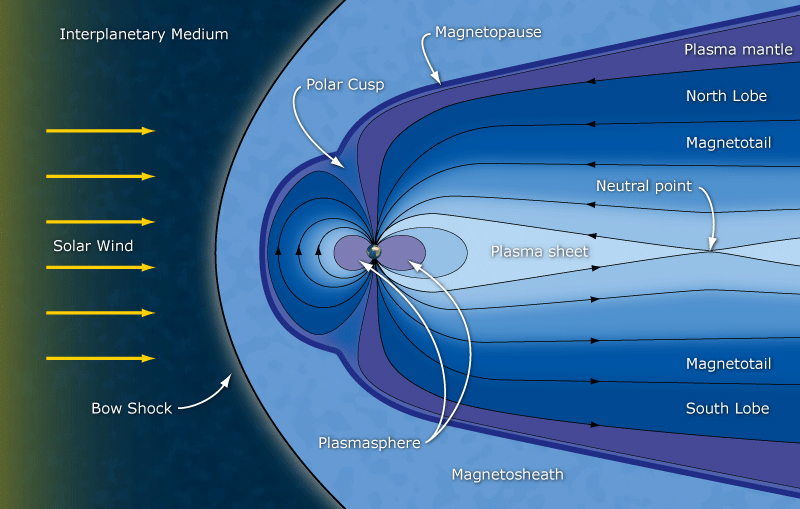
\includegraphics[scale=0.5]{{Figures/MagnetoOverview.jpg}}
	\caption{Overview of the magnetosphere and plasmasphere \citep{MagnetosphereOverallFigure}.}
	\label{RingCurrentFigure}
\end{figure}

The inner magnetosphere, where this dissertation is primarily focused, is composed of three main constituent parts: the plasmasphere, the ring current, and the radiation belts, all of which are shown in Figure \ref{fig:magnetosphereoverview}. This helps illustrate how the parts are not always spatially distinct and, depending on conditions, often overlap.


\begin{figure}[htp]
	\centering
	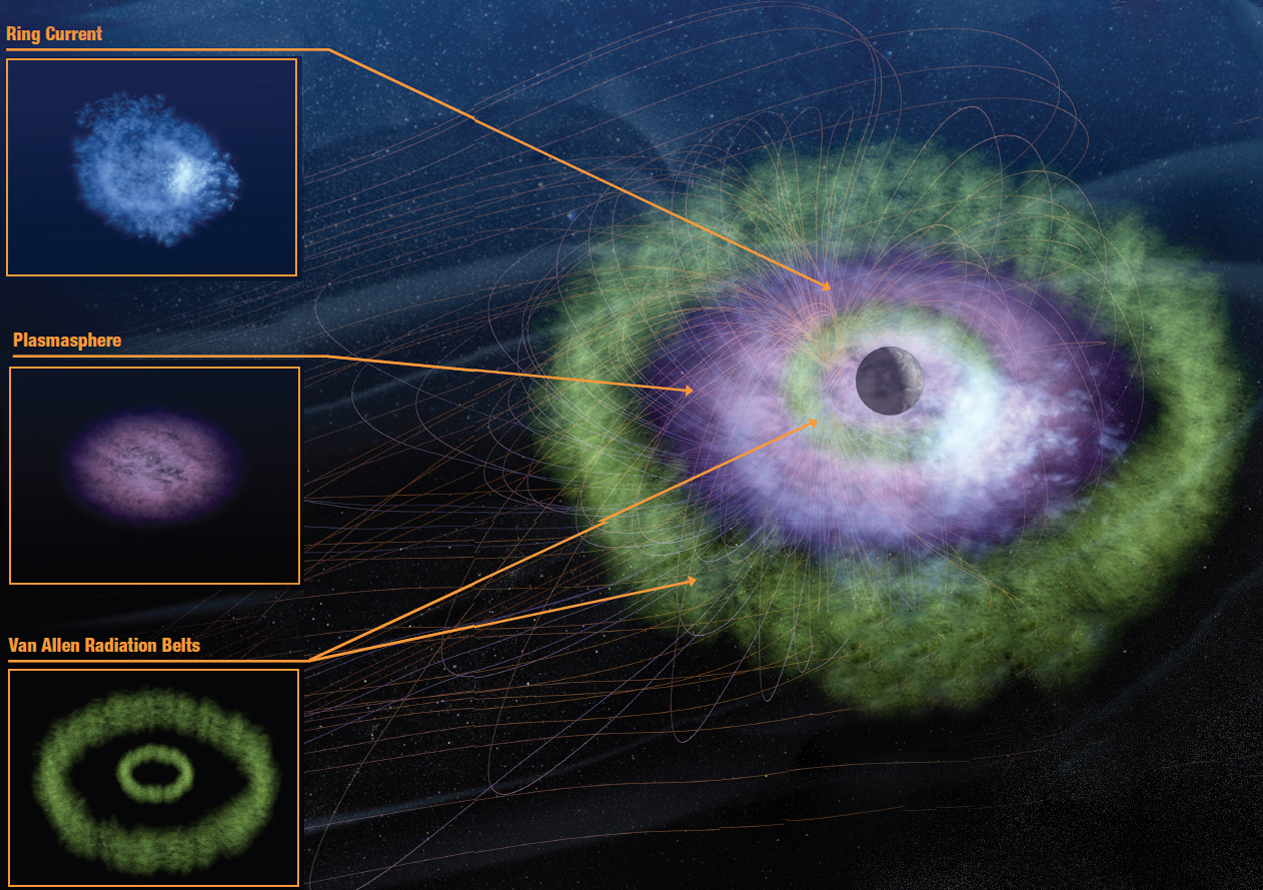
\includegraphics[scale=0.3]{{Figures/innermag-2.jpg}}
	\caption{Overview of inner magnetosphere. Adapted from \citep{InnerMagNASA}.}
	\label{fig:magnetosphereoverview}
\end{figure}



\subsubsection{Processes}

The complex structure of the magnetosphere and plasmasphere leads to a number of distinct behaviors and processes such as a ring current and geomagnetic storms and substorms, all of which are driven by the solar wind.

The Ring Current, one of the major magnetospheric currents shown in Figure \ref{RingCurrentFigure}, is composed of charged particles drifting opposite directions around the Earth based on their polarity. A schematic of this from a top-down perspective is shown in Figure \ref{fig:Gold1960DriftMotion}. With enough energetic particles drifting together, a current is generated that can significantly affect the magnetic field measured on Earth's surface. These particles in the current are energized into the magnetosphere via conditions that cause the solar wind's magnetic field to reconnect with that of Earth.

\begin{figure}[htp]
	\centering
	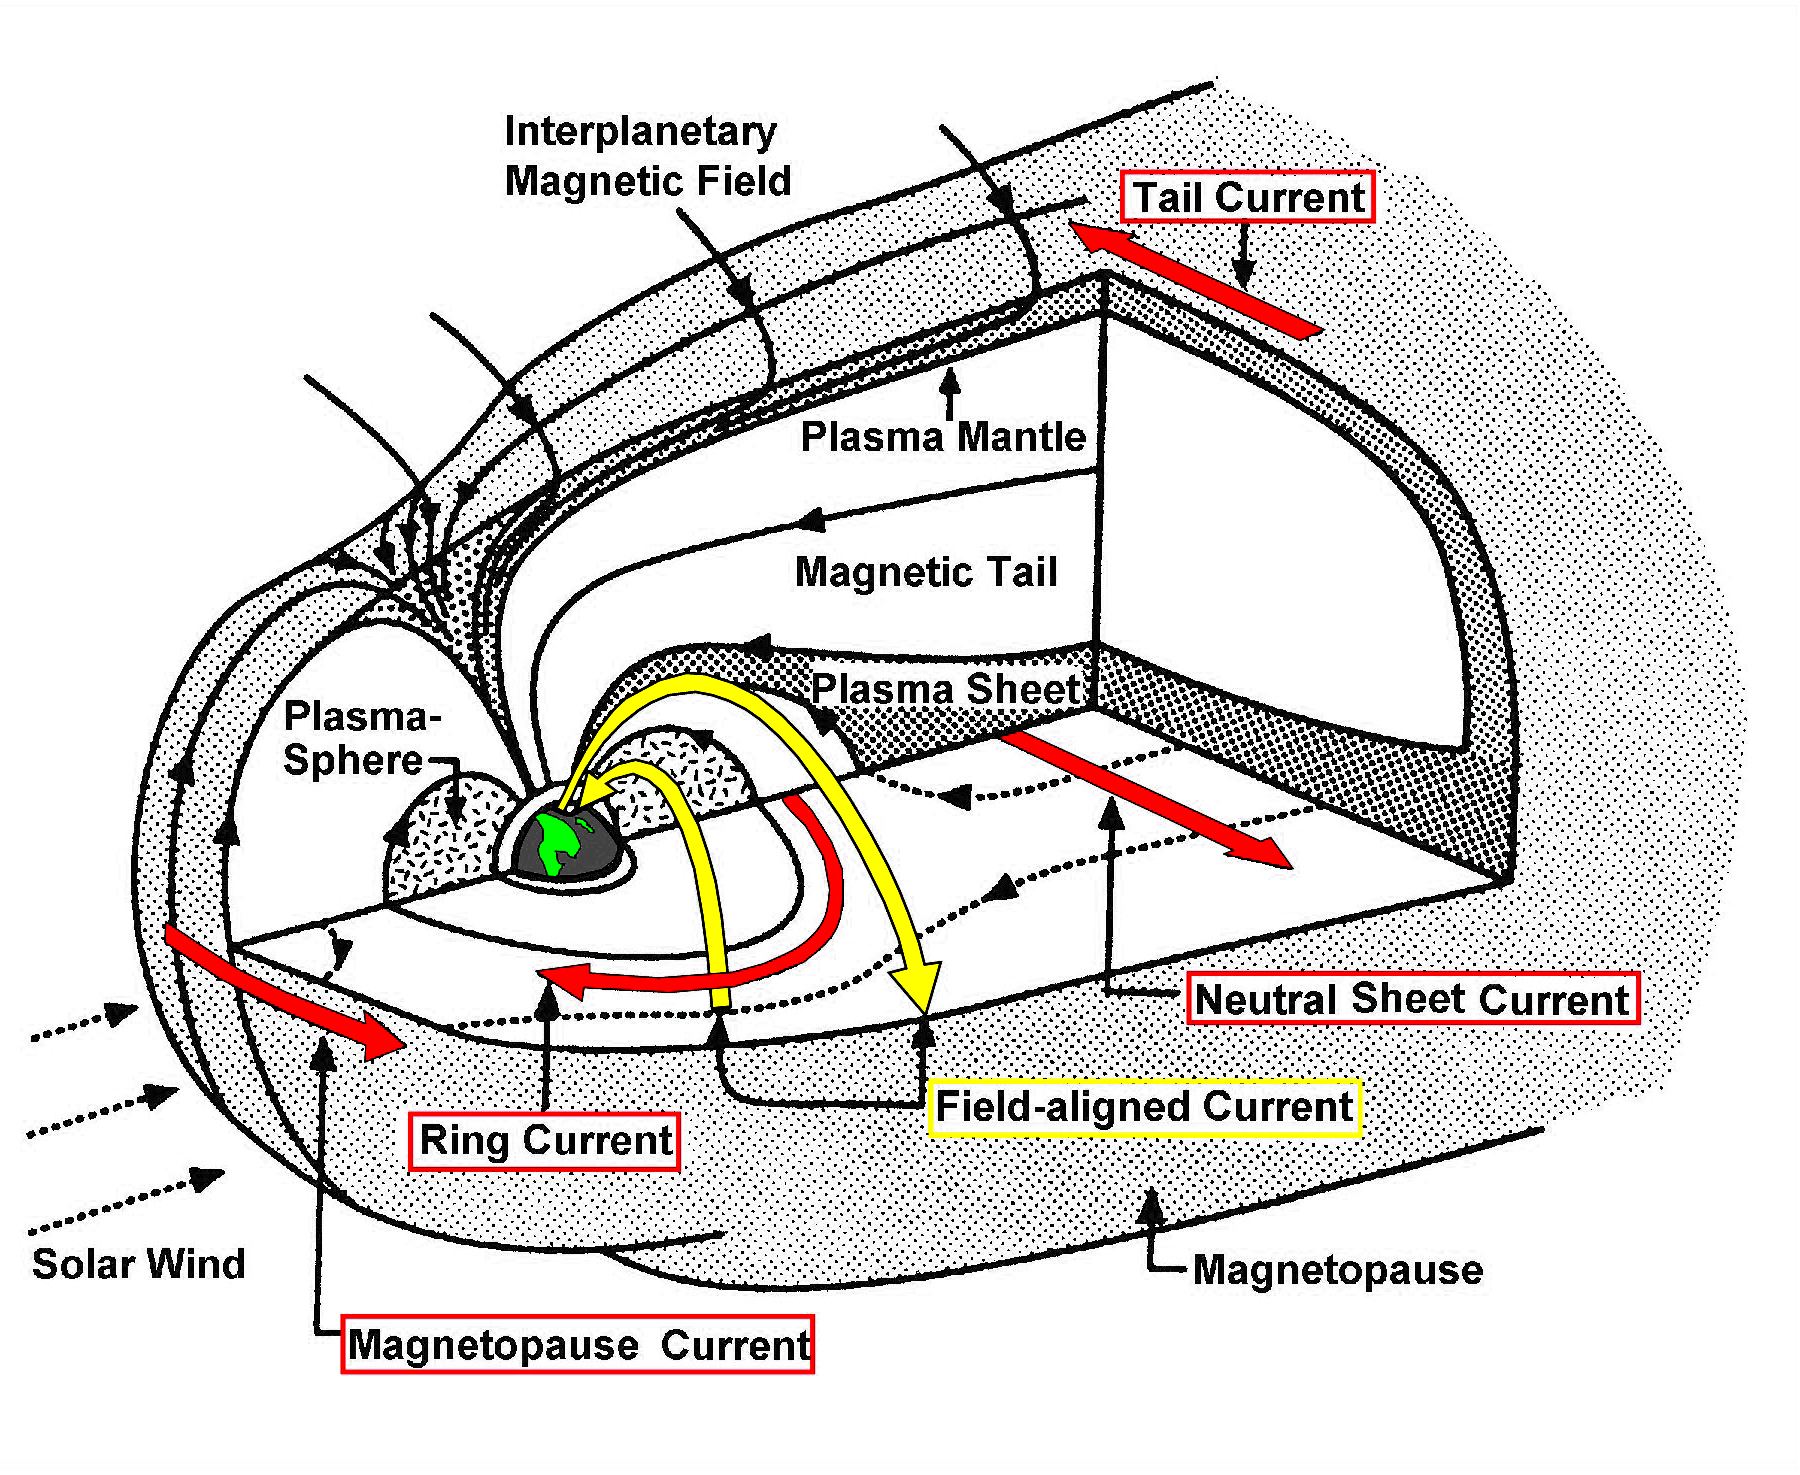
\includegraphics[scale=0.25]{{Figures/magnetosphere.jpg}}
	\caption{Currents in/around the magnetosphere. Adapted from \citep{MagnetosphereCurrentFigure}.}
	\label{RingCurrentFigure}
\end{figure}


\begin{figure}[htp]
	\centering
	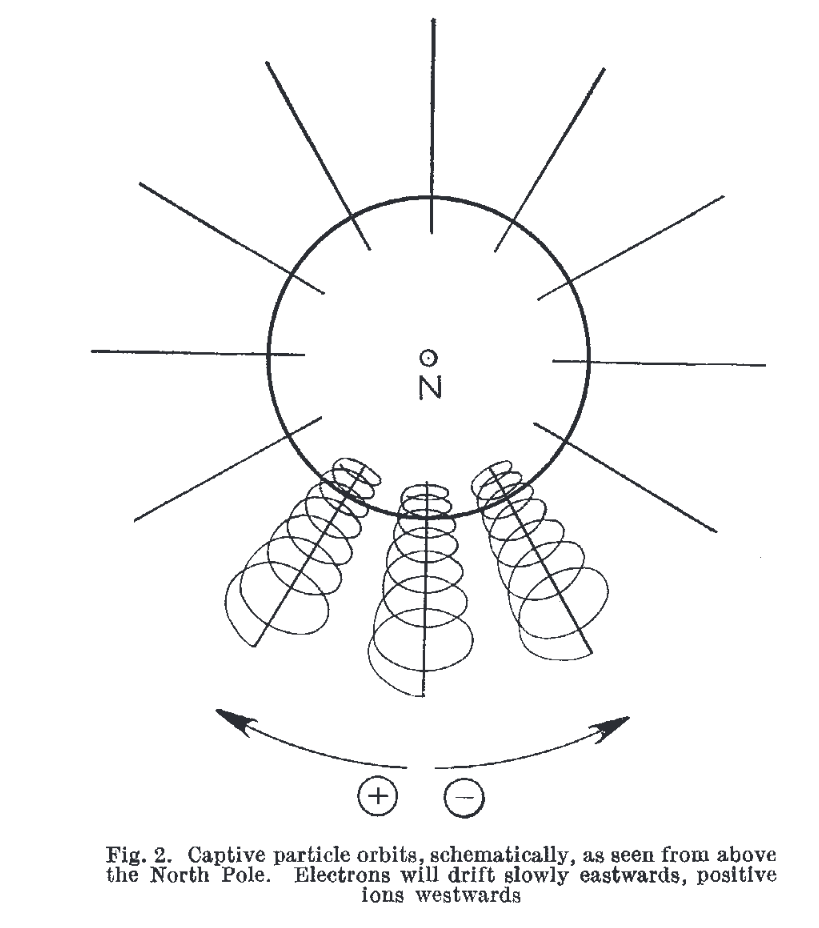
\includegraphics[scale=0.3]{{Figures/Gold1960RingCurrent.png}}
	\caption{Top-down schematic of particle drift \citep{Gold1959RingCurrent}.}
	\label{fig:Gold1960DriftMotion}
\end{figure}


Geomagnetic storms occur when the solar wind interacts with the Earth's magnetosphere in such a way as to produce significant disruptions in its normal, quiet-time, behavior. A geomagnetic storm is generally defined by a significant change to the magnetic field measured by multiple ground-based magnetometer measurements from stations spread around the world, in the case of the $K_P$ index, or around the geomagnetic equator in the case of the disturbance storm-time ($D_{st}$) index. These indices are used to classify storms into categories of severity \citep{NOAAScale}. The definition of storms in the literature varies slightly between authors \citep{Yermolaev}, but most agree that sustained and abnormally perturbed near-earth and mid-to-low geomagnetic latitude magnetic field strengths over several hours or more constitutes a geomagnetic storm \citep{StormDefinition}. 

Geomagnetic substorms, in contrast with storms, are much shorter; typically only lasting for an hour or two, and potentially happening soon after one another. They tend to have a less appreciable effect on the amount of particles/energy in the ring current, and are associated with sudden changes in energy coming from the tail of the magnetosphere rather than the dayside reconnection associated with storms \citep{Gonzalez1994WhatIsAStorm}. Figure \ref{fig:alldata-GOES6-1989-1989} serves as an example of this, where a long, high-intensity storm is punctuated with a few small, short disturbances in both $B_z$ and \dst.

\begin{figure}[htp!]
	\centering
	\includegraphics[width=1\linewidth]{Figures/alldata-GOES6-10Mar1989-17Mar1989.eps}%alldata-GOES6-1989-1989}
	\caption{Data from GOES 6 around March 1989 geomagnetic storm.}
	\label{fig:alldata-GOES6-1989-1989}
\end{figure}



Geomagnetic storms and substorms can have significant impacts on Earth and space systems, from inducing currents in large power grids to harming satellite circuitry and onboard data \citep{1989Storm}. Because of the potential damage of such events, any ability to forecast a storm could allow operators to prevent or mitigate problems in their systems. Because of the large correlation of CMEs with geomagnetic storms \citep{Yermolaev}, it can be estimated that our forewarning time is the difference between observing a CME (via visual or X-ray methods) and its propagation time plus magnetospheric interaction time. This time can span from one to five days, depending on the speed of the CME and how it interacts with the interplanetary medium \citep{StormSources}. 

All of these processes are coupled to some degree with the plasmasphere, by transferring plasma and energy from the interplanetary medium to near-Earth regions ($\lesssim 8 R_E$). 


\subsection{Radiation Belts}

\subsubsection{Discovery}
The radiation belts that surround Earth, known as the Van Allen Radiation Belts, are two (occasionally three \citep{LinksBetweenPlasmapauseRadiationBelt}) bands of energetic particles encircling the planet. The existence of such bands was theorized based on knowledge of magnetically trapped motion of charged particles; results from rocket soundings showed that more radiation exists in the auroral regions than at the equator.  The beginning of the space age allowed particle counters to be launched onboard the Explorer 1 and Explorer 3 satellites, which found radiation far beyond what was anticipated and concentrated into bands of high intensity \citep{MagnetoHistory}.

\subsubsection{Processes}
The outer radiation belt is filled with electrons captured from the solar wind by the magnetosphere and then injected into the radiation belts from the magnetotail, and occasionally lost when the magnetopause moves back Earthward \citep{Millan2007ReviewRadiationElectronLoss}. The inner belt tends to be filled by heavier species from the ionosphere, and is overall less variable than the outer belt \citep{LinksBetweenPlasmapauseRadiationBelt}. It gains particles from inward radial diffusion and loses them to the atmosphere via plasmaspheric hiss \citep{Lyons1973StructureRadiationBelt}. The slot region between the two is formed by the interaction of energetic particles with very low frequency (VLF) waves, leading to particle loss to the atmosphere \citep{LongTermVariationsSlotRegion}. In contrast to the ring current particles, the radiation belt particles tend to have much higher energy.

\begin{figure}[htp]
	\centering
	\includegraphics[scale=0.15]{{Figures/BounceMotion.eps}}
	\caption{Motion of magnetically trapped particles \citep{IntroductionToGeomagneticallyTrapped}.}
	\label{BounceMotion}
\end{figure}

The various forms of particle movement are shown in Figure \ref{BounceMotion}. The primary component being the drift motion leading to the ring current. As particles approach the ``Mirror point", a slight angle between the guiding center motion and the magnetic field line leads to a force opposing the motion along the line, eventually mirroring the particle back in the opposite direction. Because mirroring applies to all particles within a certain range of energies and pitch angles, the collective sum of trapped particles forms the radiation belts. By modeling the particle mass, momentum, and the magnetic field strength of a given dipole magnetic field, approximations can be made regarding the amount of particles that will become trapped in the field, and the amount that will be lost to scattering \citep{Young2008MagneticFieldLineCurvature}.

The radiation belts have an impact on the plasmasphere by acting as an occasional source of low energy particles and a sink for high energy particles. The plasmasphere also acts on the radiation belts via the VLF waves, energizing electrons out of the plasmasphere and into the radiation belts, or providing particles already in the belts the energy needed to become untrapped \citep{LinksBetweenPlasmapauseRadiationBelt}. While the outer limits of the plasmasphere and the outer radiation belt often coincide and react similarly to geomagnetic activity, they can become separated during geomagnetically active times \citep{LinksBetweenPlasmapauseRadiationBelt}. An example of this variation in relative position is shown in Figure \ref{PlasmasphereRadiationBeltFig}.

\begin{figure}[htp!]
	\centering
	\includegraphics[scale=0.15]{{Figures/Cluster_plasmasphere.eps}}
	\caption{Relative position of plasmasphere (blue) and radiation belts (red) with varying geomagnetic activity levels \citep{LinksBetweenPlasmapauseRadiationBeltFig}.} 
	\label{PlasmasphereRadiationBeltFig}
\end{figure}

Another source/sink of energy for particles in the radiation belts (or general magnetospheric plasma) is via Alfvén waves \citep{Keling2009AlfvenWaves}. These waves are composed of oscillating electromagnetic fields carrying both energy and field-aligned currents (via oscillating electrons) as they propagate. By moving energy along the field lines, Alfvén waves also couple the various distinct regions of plasma around Earth. 


\subsection{Plasmasphere}

\subsubsection{Discovery}
The plasmasphere, shown in Figure \ref{fig:magnetosphereoverview}, was largely unknown until the beginning of the space age, being found both through analyses of very low frequency radio waves and in-situ spacecraft measurements. Previously, it was believed that electron density decreased continuously from the ionosphere to the interplanetary medium \citep{LemaireEarthsPlasmasphere}. These measurements showed that the Earth had a sphere of cold plasma around it that ended in an abrupt boundary, and varied in location and density gradient with geomagnetic activity \citep{Carpenter1966WhistlerStudiesPlasmapause,LemaireEarthsPlasmasphere}.

\subsubsection{Processes}
The plasmasphere is interconnected with the radiation belts and the ionosphere. While many of the specifics of this interaction are still not fully understood, some parts have been observed and explained to a reliable degree of accuracy. 

In the ionosphere, sunlight photoionizes oxygen which produces excess electrons that are transferred up via polar wind into the plasmasphere along magnetic field lines bringing energy and heat along with it. This daily ``refilling"  flux continues until a saturation point is reached, bringing the lower bounds of the plasmasphere into equilibrium with the upper ionosphere. This flux also typically reverses on the night side, sending electrons back down into the ionosphere \citep{LemaireEarthsPlasmasphere}. Figure \ref{fig:PlasmasphereRefilling} shows one particular example of active geomagnetic conditions emptying the plasmasphere following by a quiet time refilling flux restoring density over a couple of days.

\begin{figure}[htp]
	\centering
	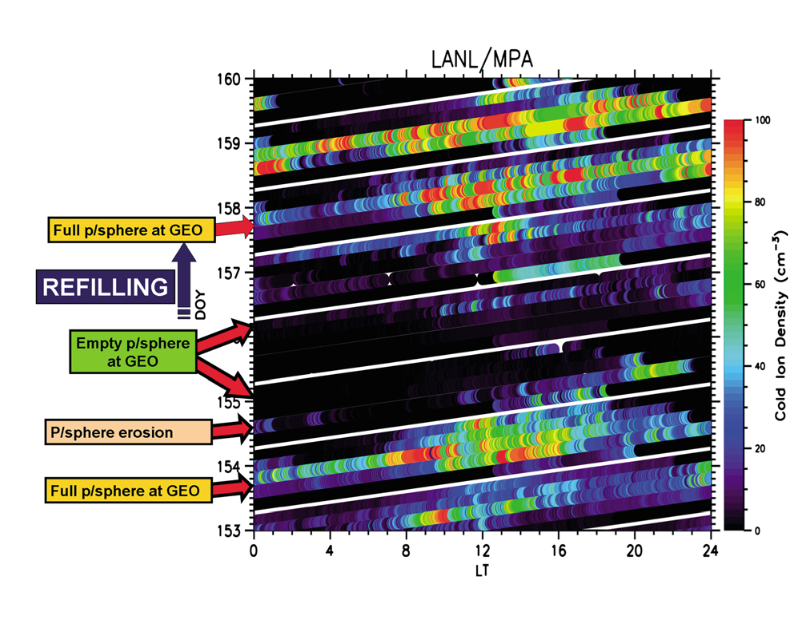
\includegraphics[scale=0.4]{{Figures/PlasmasphereRefillingT.png}}
	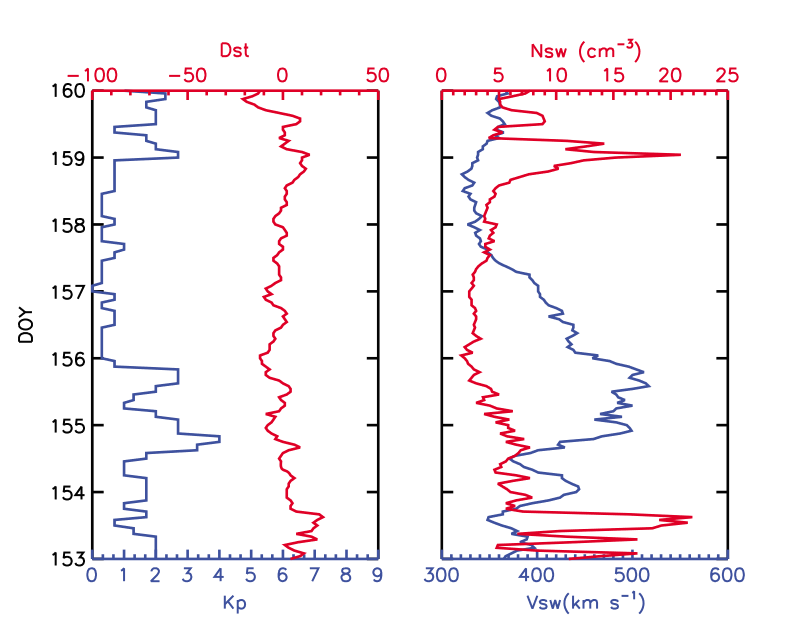
\includegraphics[scale=0.4]{{Figures/PlasmasphereRefillingB.png}}
	\caption{Plasmasphere ion density emptying and refilling as measured by GEO in 2007, along with coinciding solar wind conditions. From \citep{Denton2014ObservationsModelingRefilling}.}
	\label{fig:PlasmasphereRefilling}
\end{figure}


During periods when the location of the plasmapause is quickly brought earthwards, or the plasmapause is re-established in a new location, plasma left outside the plasmapause is known to be magnetically convected outwards and sunwards \citep{ErosionRecoveryPlasmasphere, LemaireEarthsPlasmasphere}, termed ``eroding" the plasmasphere. This is because the location of the plasmapause can vary greatly with geomagnetic conditions. Figure \ref{fig:LemaireKnee} shows how the $L$-shell distance varies with magnetic activity via the $K_p$ index.

\begin{figure}[htp]
	\centering
	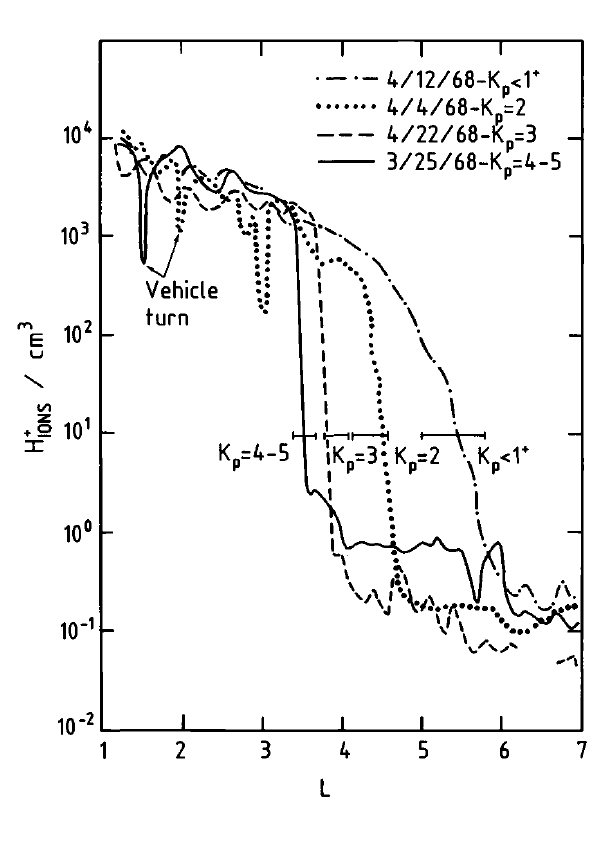
\includegraphics[scale=0.65]{{Figures/LemairePlasmapauseKnee.png}}
	\caption{Plasmapause position varying with $K_p$ as represented by several particular plasmapause crossings made on outbound passes between local times of midnight and 0400 \citep{LemaireEarthsPlasmasphere}.}
	\label{fig:LemaireKnee}
\end{figure}

Figure \ref{fig:LemaireKnee} also shows the plasmatrough; the low density region just outside the plasmapause where particle count often drops multiple orders of magnitude from the plasmasphere and continues out through the magnetosphere. The location of what is called the "plasmapause knee" varies with time and geomagnetic activity, where the dayside boundary is often less steep than the nightside boundary. It is also observed in Figure \ref{fig:LemaireNoKnee} that after multiple days of quiet geomagnetic conditions, the saturated plasmasphere smooths the knee out until the plasmapause is almost unidentifiable \citep{LemaireEarthsPlasmasphere}. 

\begin{figure}[htp]
	\centering occasional 
	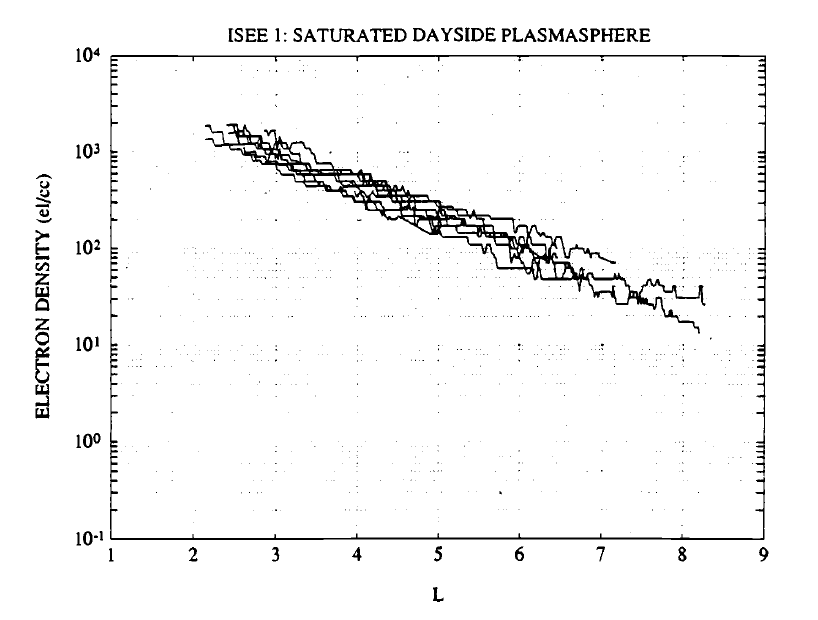
\includegraphics[scale=0.5]{{Figures/LemaireQuietPlasmapause.png}}
	\caption{Multiple ISEE 1 passes made between 09-15 MLT during saturated plasmapause conditions \citep{LemaireEarthsPlasmasphere}.}
	\label{fig:LemaireNoKnee}
\end{figure}


At times, the plasmasphere becomes distorted at the plasmapause due to dayside reconnection, causing bulges that can become elongated and detached during co-rotation, usually on the dusk side. These extended segments of plasma are known as ``plumes" and appear as a peak in density in a normally empty plasmatrough. These plumes also often occur with, and possibly because of, enhanced magnetospheric activity \citep{EvolutionPlasmasphericIons}. This bulge, and the effects of geomagnetic activity on the bulge, is shown in Figure \ref{fig:plasmabulge}

\begin{figure}[htp]
	\centering
	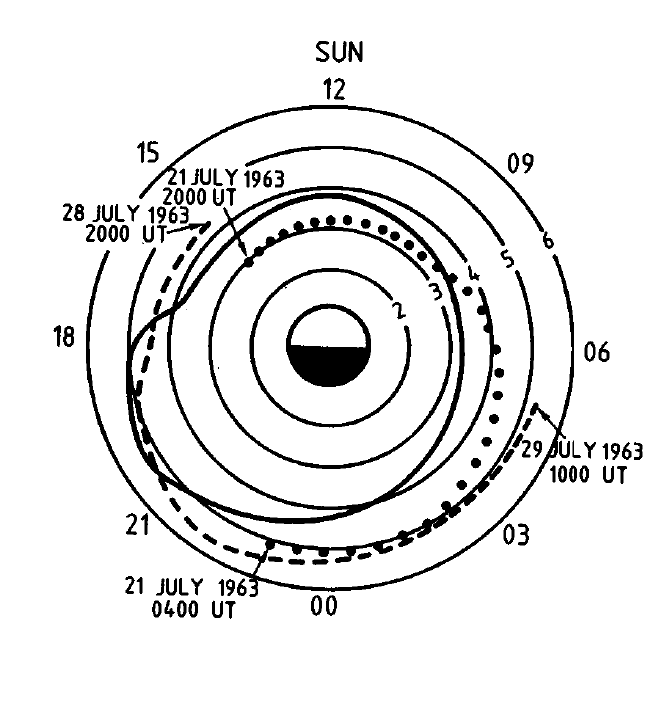
\includegraphics[scale=0.5]{{Figures/LemairePlasmapauseRadius.png}}
	\caption{Plasmasphere dusk-side bulge with geomagnetic activity. The solid line is the average position of the plasmasphere knee during periods of $K_p=2-4$, while the dots indicate a specific instance of increasing magnetic activity, and the dashes a specific instance of decreasing activity \citep{LemaireEarthsPlasmasphere}.}
	\label{fig:plasmabulge}
\end{figure}

What is not particularly well studied or understood is the behavior of plasma mass density in the plasmatrough. Most studies focus on behavior inside the plasmapause where density is higher and easier to measure, but since this mass diffuses inwards from the solar wind and through the plasmatrough, and satellites are often located in the plasmatrough (geostationary equatorial orbit (GEO) is at about 6-7 $R_E$), it is worthwhile understanding the behavior of the region. This work takes a dataset specifically focused on mass density in the plasmatrough and attempts to understand, classify, and forecast behavior as it relates to solar wind and geophysical conditions.


\subsection{Statistical Modeling of Magnetosphere and Plasmasphere}

Initial forecasts of geomagnetic disturbances were based on an observed time delay from sunspot sightings \citep{SunspotStorms}. The state of geomagnetic storm forecasting then advanced to a basic theory involving electromagnetic interactions in the magnetosphere \citep{Chapman}. There now exist entire services dedicated to executing statistical and magnetohydrodynamic (MHD) based models of the magnetosphere \citep{CCMC}, as well as multi-year, multi-institution efforts to survey the general statistics of modeling and forecasting of extreme events \citep{ExtremeEvents}.

The convergence of the advancement in both statistical and MHD-based simulation has led to a situation where the scientific community has the capacity for monitoring and forecasting the near-Earth effects in real time.  There have been efforts to test the forecast performance of select models over a small number of geomagnetic events \citep{ANNforecast,StormModel,StatCompStorms,Yermolaev, GEMPapers}. However no research has been done that involves the analysis of long-term forecasting performance of these models and comparison of the results with existing methods.

Three main metrics of magnetospheric activity are seen throughout the literature; the $K_p$ index: a measure of magnetosphere convection caused by currents induced by a changing plasma sheet (and indirectly from the global convection field strength) \citep{Thomsen2004WhyKpSoGood}; the $AE$ index: a measure of electrojet activity based on the maximum and minimum field strength measurements from magnetometer stations at auroral latitudes \citep{DavisSugiura1966AE}; and the previously mentioned $D_{st}$ index based on magnetic field perturbations caused primarily by a changing ring current. All three indices are derived from a set of ground stations shown in Figure \ref{fig:GroundStations} based on the nature of the metric.

\begin{figure}[htp]
	\centering
	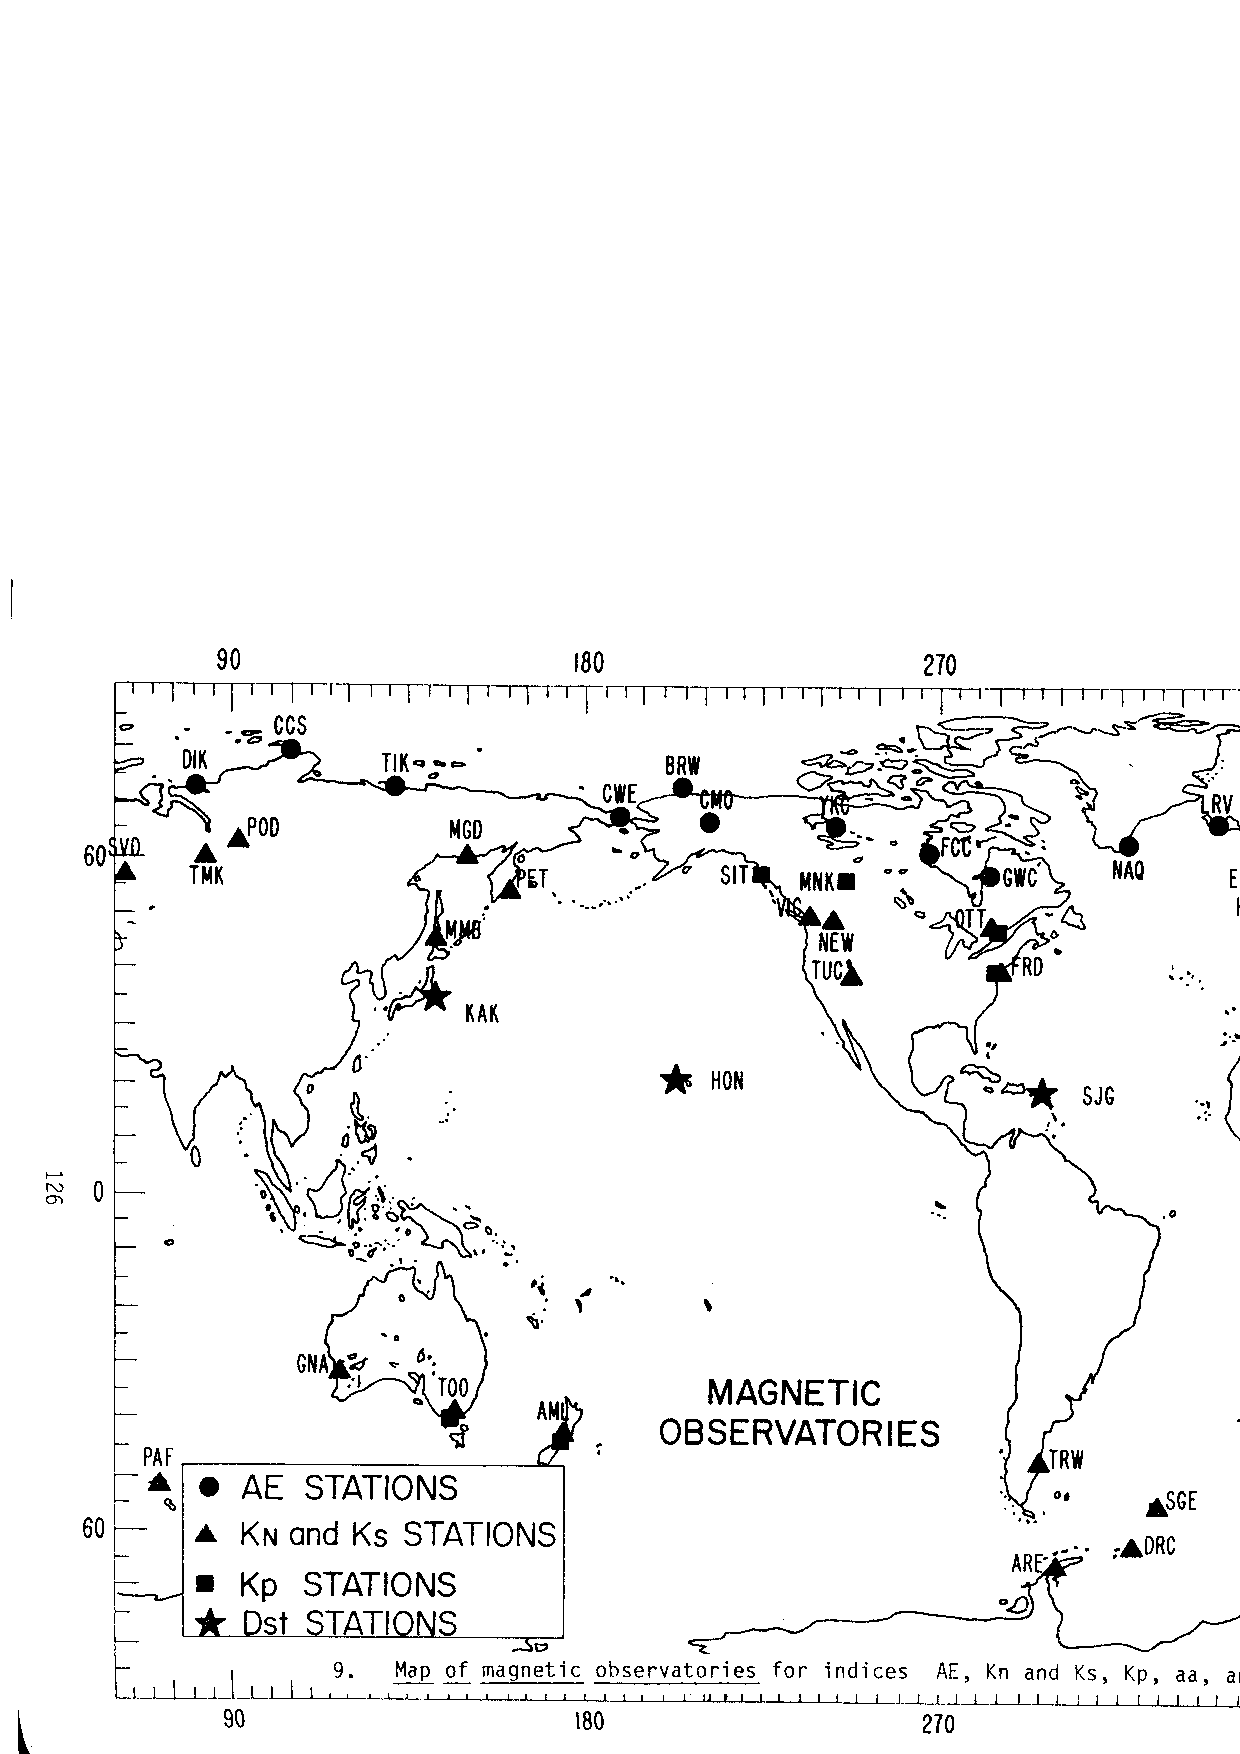
\includegraphics[scale=0.5]{{Figures/StationMap.pdf}}
	\caption{Map of ground stations used to measure the $K_p$, $AE$, and \dst\ indices \citep{CommonMagneticIndices}.}
	\label{fig:GroundStations}
\end{figure}


Models specific to the plasmasphere and plasmatrough include Carpenter and Anderson's ISEE/Whistler Model of Equatorial Electron Density in the Magnetosphere, which use empirical data to determine the location and density of the saturated plasmasphere and plasmatrough \citep{Carpenter1992ISEEModel}. \cite{Carpenter1992ISEEModel} analyze ISEE 1 data for drops in number density of at least a factor of 5 across half an L-shell and state that the inner edge of the plasmapause is located at $L_{ppi}=5.6-0.46K_{p_{max}}$. Here $K_{p_{max}}$ is the maximum value of $K_p$ (an index averaging 11 mid-latitude stations in the previous 24 hours), and $L$ is the set of magnetic field lines at a distance of $L$ Earth radii at the magnetic equator. This specifies the outer boundary of the plasmasphere, and from there the density is modeled inwards as $n_e=n_{e_{L_{ppi}}}\cdot 10^{-(L-L_{ppi})/\Delta pp}$, where $n_{e_{L_{ppi}}}$ relates day number, sunspot number, whistler profiles, and multiple year-long perturbations in an exponential fashion shown as $n_e(L,d,\bar{R})=10^{\Sigma x_i}$. $L_{ppi}$ and $\Delta pp$ are empirically derived plasmapause location and width, respectively. $x_1$ is a whistler reference profile, and indices $i=2-4$ represent perturbation values for annual, semiannual, and solar cycle variations respectively. The exact numbers in the density profiles vary slightly between a midnight-06 MLT model, and a 06-15 MLT model, based on the specific passes used to fit the parameters for each section. 

\cite{Gallagher2000GlobalCore} created a Global Core Plasma Model which combines empirically derived models of the ionosphere, plasmasphere, and magnetosphere. For the plasmasphere it links plasma density and magnetosphere conditions by fitting Carpenter's equation, but replacing their piecewise dependence on MLT with a sinusoidal term along with extra factors to account for the post-dusk bulge while still keeping the plasmasphere model continuous. At the most basic level, the plasmasphere component reduces to an exponential equation of the form $n_{ps}=10^{gh}-1$, where $g$ and $h$ are terms relating to the inner plasmasphere and plasmapause, combining sunspot number, day of year, and a plasmapause gradient term that accounts for the MLT dependence in the form of $\Delta_{pp}=0.036\cdot \sin(\frac{2\pi (MLT-6)}{24})+0.14$. They also link plasmasphere filling time to $K_p$, stating it starts at 3.5 MLT and fills until a time of $\Phi_{TP}=0.145K_p^2-2.63K_p+21.86$ hours \citep{Gallagher1995AzimuthalVariation}.

\cite{Moldwin2002ModelPlasmapause} build on Carpenter's model by taking CRRES data and the same plasmapause detection parameters as Carpenter, finding 969 plasmapause detections compared to the 40 used to derive the model in \cite{Carpenter1992ISEEModel}. Using the abundance of data they do statistical analyses such as showing a least squares linear fit between increasing $K_p$ and decreasing L-shell of the plasmapause of the form $L_{pp}=(5.39\pm 0.072)-(0.382\pm 0.019)\cdot K_p(max)$ with a correlation of 0.548. They also find that if they limit this to plasmapause crossings between 09 and 15 MLT, the linear correlation increases to 0.727.

\cite{OBrien2003EmpiricalPlasmapause} find that using auroral electrojet (AE) or disturbance storm time ($D_{st}$) indices work better than $K_p$ for determining plasmapause location. They use the same plasmapause crossings as \cite{Moldwin2002ModelPlasmapause} and model them against hourly changes in the ring current (via $D_{st}$) or 1-minute changes
 in the auroral electrojet currents ($AE$). They take the maximum (or minimum, as required) of each index over a varying range of hours, from a start of up to 72 hours before crossing up to end of at least 6 hours before crossing, and fit a basic linear model. Their three best models were a basic linear fit of $L_{pp}$ to $\text{max}_{-36,-2}K_p$, $\text{max}_{-36,0}AE$, and $\text{log}_{10}(\text{min}_{-24,0}D_{st})$. Using a bootstrap analysis for significance, all three models were indistinguishably similar in the root mean square error (RMSE) of their respective models, except for $AE$ having significantly less error in the night sector than $D_{st}$. Making the model slightly more advanced by including a MLT dependence and periodic terms allows a bulge to be approximated, and finds that the allowing local time to be accounted for significantly (at the 95\% confidence level) reduces the error of the model, but still shows no significant difference between models of the same complexity.

\cite{Denton2006} models the distribution of electrons along magnetic field lines based on measurements from the Radio Plasma Imager onboard the IMAGE spacecraft. They attempt to show that mass density has a local peak near the magnetic equator, and do show that in some cases it can be inferred, especially for values of $L \ge 6$, but can not conclusively establish its existence. 

As for models specifically of the plasmatrough, \cite{Lotoaniu1999PlasmaMassDensity} take ground based Ultra Low Frequency (ULF) wave measurements, then map them to plasma mass densities between $L=4.5$ and $L=10$ via the Tsyganenko T89 magnetic field model and an $R^{-4}$ plasma mass density profile. These estimated values were then compared to in-situ measurements from the CRRES satellite and found that this technique can, under specific conditions where all of the field lines at the ground stations map to plasmatrough, accurately measure plasmatrough mass density. 

\cite{Takahashi2006MassDensityInferred} take a similar approach, but approximate ULF waves from the CRRES satellite directly, instead of using ground stations, and then map that to mass density values. By using the electric field spectra on the satellite and finding a fundamental frequency of the toroidal waves, they estimate mass density with a combination of theoretical model and empirical observations. The magnetic field model used is either T89 or T96, dependent on $K_p$ or \dst\  respectively. Instead of an $R^{-4}$ dependence for the mass density model, they use $\rho=\req(LR_E/R)^{0.5}$, and then combine with frequency observations via $\rho_{eq\_est}=\rho_{eq\_theory}(f_{1\_theory}/f_{1\_obs})^2$.

\cite{Takahashi2010SolarCycleVariation} similarly looks at deriving mass density using toroidal Alfvén waves, but switch from using the fundamental harmonic mode to using the third harmonic because it was most detectable at the location of the GOES satellites, which they used in place of CRRES to get a geostationary orbit and larger number of observation points. The methods are largely the same as the previous paper, but include statistics accounting for detection rates of $f_{T3}$ and slight modifications to technique required for the geostationary satellites.

\cite{Min2013} derives equatorial mass density using the GOES and AMPTE satellites by applying magnetoseismology to the toroidal Alfvén waves, confirms the benefits of using the third toroidal frequency as described by Takahashi and Denton, and confirm the statistical properties of the dataset such as $f_{T3}$ being largely undetectable in the midnight region and the high correlation between \req\ and \f.

\cite{Denton2015FieldLineDist} also uses the GOES satellites to determine mass density at geostationary orbit. They assume the same form of power law as \cite{Takahashi2006MassDensityInferred} but with a fit power parameter $\alpha$, making the equation: $\rho=\req(LR_E/R)^{\alpha}$, then normalize to the third harmonic frequency for data availability. Binning by harmonic frequency, they fit Gaussian curves to MLT, \f, and $AE$ to get best fit $\alpha$ for the model, and end up getting a model that produces a good average value for field line density.

Most of these studies focus on plasma density in the plasmapause and plasmasphere, since that is where the densities are the highest, easiest to measure, and have the most data availability. This study focuses on the plasmatrough partly due to its unexplored nature, and largely due to the significance of the region to objects in geostationary orbits. It also couples with both the magnetosphere and plasmasphere, suggesting that a greater understanding of the behavior of the plasmatrough may aid in understanding the coupling of both major bordering regions.





\chapter[Models]{Methods}

This work utilized a number of linear and nonlinear methods of analysis and modeling, including Auto-Regressive Moving Average models with eXogenous inputs (ARMAX) and neural net models. No single method is ideal, and using many methods is better for insight, especially for nonlinear/complex systems. The details of their application will be expanded upon in their respective sections.

\section{Linear}

\subsection{Overview}
Due to its simplicity and ease of application, linear models are used in practically all fields as a first attempt to discover information about the data and any potential relationships. In Space Physics, where the underlying behavior of a complex system is not theoretically known, and in-situ measurements are sparse, linear models are often the first step towards understanding what components are related and to what degree. Sometimes this leads to understanding unexpected complexities in a system.
\vnote Example. Lemaire p.183 heavier ions in outer plasmasphere than inner plasmasphere? Correlation between plasmapause and radiation belt boundary?

\subsection{ARX}

Impulse response systems are systems in which the output (a response) is driven by a linear sum of coefficients of an input (a series of impulses). A simple example would be making a loud noise in a concert hall. The response will be the unique echoes and reverberations created by the initial driving sound, and with enough signal, a statistical model can be generated that will map the input sound to a response echo. In the magnetosphere, the most used example is an impulse of $v_{B_s}$ driving the Auroral Electrojet (AE/AL) index \citep{VBzAL}, or the Disturbance Storm Time ($D_{st}$) index \citep{VBzDST}, also shown in Figure \ref{VBzIRplot}.

\begin{figure}[htp]
\centering
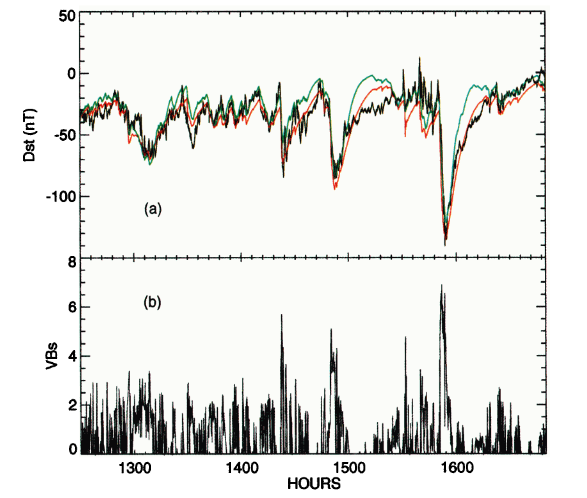
\includegraphics[scale=0.40]{{Figures/VBzIR.png}}
\caption{DST (black), nonlinear autoregressive exogenous (ARX) model (red), Burton et al 1975 model (green). (b) $v_{B_S}$ impulse as input \citep{ARXEqn}}
\label{VBzIRplot}
\end{figure}

This plot shows how different models are used to predict magnetospheric variables with varying amounts of success. In this proposal, what starts as a simple Box-Jenkins model of the form \citep{DOYvar}:
\begin{align*}
x(t)&=c+\sum_{j=0}^{m}{a_j f(t-j\Delta t)}
\end{align*}
can be modfied with an auto-regressive component to be an autoregressive model with exogenous inputs (ARX) such as that used in \cite{ARXEqn}, taking the form:
\begin{align}
\hat{x}(t+\Delta t)&=\sum_{i=0}^la_i\cdot x(t-i\Delta t)+\sum_{j=0}^m b_j\cdot f(t-j\Delta t)+c
\label{ARXEqn}
\end{align}
Where $m$ and $l$ are the number of coefficients desired for including previous data points in the prediction, and $c$ is a factor to remove the mean offset from the data. Note that in some cases the starting value of the iterators can be individually increased if there is a known delay in response time or there is a desire to predict further into the future. In \cite{ARXEqn}, second order equations ($m=2$) were used with anywhere from one to four driving coefficients, but in practice any number of coefficients and any number of driving variables can be used up to some fraction of the number of data points that allows the coefficient matrices to be solved for. 

There generally is a limit to the usefulness of large-lag data \cite{ExtremeEvents}. By looking at a plot of the cross correlation relative to the number of coefficients, a limit will generally be seen where adding more coefficients no longer reduces error in the model. By creating a threshhold of change in fit per coefficient added (perhaps via a bootstrap method), the minimum number of coefficients needed to optimally model the system can be determined.

By constructing a linear system of equations from Equation \ref{ARXEqn}, the coefficients can be solved for in a general matrix form (where, in this case, $l=m$):
\[
\left( \begin{array}{ccccccc}
x_0 & ... & x_{l-1} & f_0 & ... & f_{l-1} & 1\\
x_1 &     & x_l & f_l &  &f_l & 1\\
... &     &     &     &  &   & \\
x_{N-l} & ... & x_{N-1} & f_{N-l} & ... & f_{N-1} & 1
\end{array} \right)
\left(\begin{array}{c}
a_0\\...\\a_{l-1}\\b_0\\...\\b_{l-1}\\c
\end{array}\right)
=
\left(
\begin{array}{c}
x_l \\ x_{l+1} \\ ... \\ x_{N}
\end{array}
\right)
\]

This is a linear model for the behavior of a system. However, it has been shown that the set of coefficients describing the response of a system can change with storm intensity \cite{ARXEqn}, the time scale modeled \cite{Coupling}, and even the time of day \cite{VBzAL}. This creates a very large number of possible directions for research, from predicting storm onsets, to predicting storm intensities, to modeling the overall shape and behavior of a storm, as well as all of the other possible interactions outside of storm-time. 


\subsection{ARMAX}

A class of model known as an Auto-Regressive Moving Average with eXogenous inputs model (ARMAX) is often used in time series analysis to combine the effects of persistence, linear dependence, and an average that changes with time. It makes a slight change on the ARX model in Equation \ref{ARXEqn}, adding the moving average term:
\begin{align}
\hat{x}(t+\Delta t)&=\sum_{i=0}^la_i\cdot x(t-i\Delta t)+\sum_{j=0}^m b_j\cdot f(t-j\Delta t)+\sum_{k=0}^n c_k\cdot g(t-k\Delta t)+c_{t+\Delta t}
\label{ARMAXEqn}
\end{align}


\subsection{Applicability}
As implied by the name, an ARMAX model is suitable for analysis of a time-dependent linear system where the value of a measurement is determined by its own persistence, an external variable, and some factor that contributes to a moving average with time. Most linear systems can be encapsulated by this framework, some even being overspecified with this level of accounting for variability.

\subsection{Caveats and Biases}
There will be a number of things that, ideally, must come together to make this kind of data prediction work. For one: ARX methods can often be heavily dependent on a concept known as "persistence", whereby the best prediction for a variable at any time is that same variable at the last measured time step. For example, if the high temperature today is $70^\circ$, it is fairly likely that the high temperature tomorrow will be near $70^\circ$. Too much reliance on persistence forecasting, though, and predictions can lose their usefulness. Figure \ref{persist}, for example, shows how a model can achieve high correlation with persistence, but be almost entirely useless for predicting events before they happen since the spikes are never anticipated, just modeled after they've already been seen. 

\begin{figure}[h!]
	\centering
	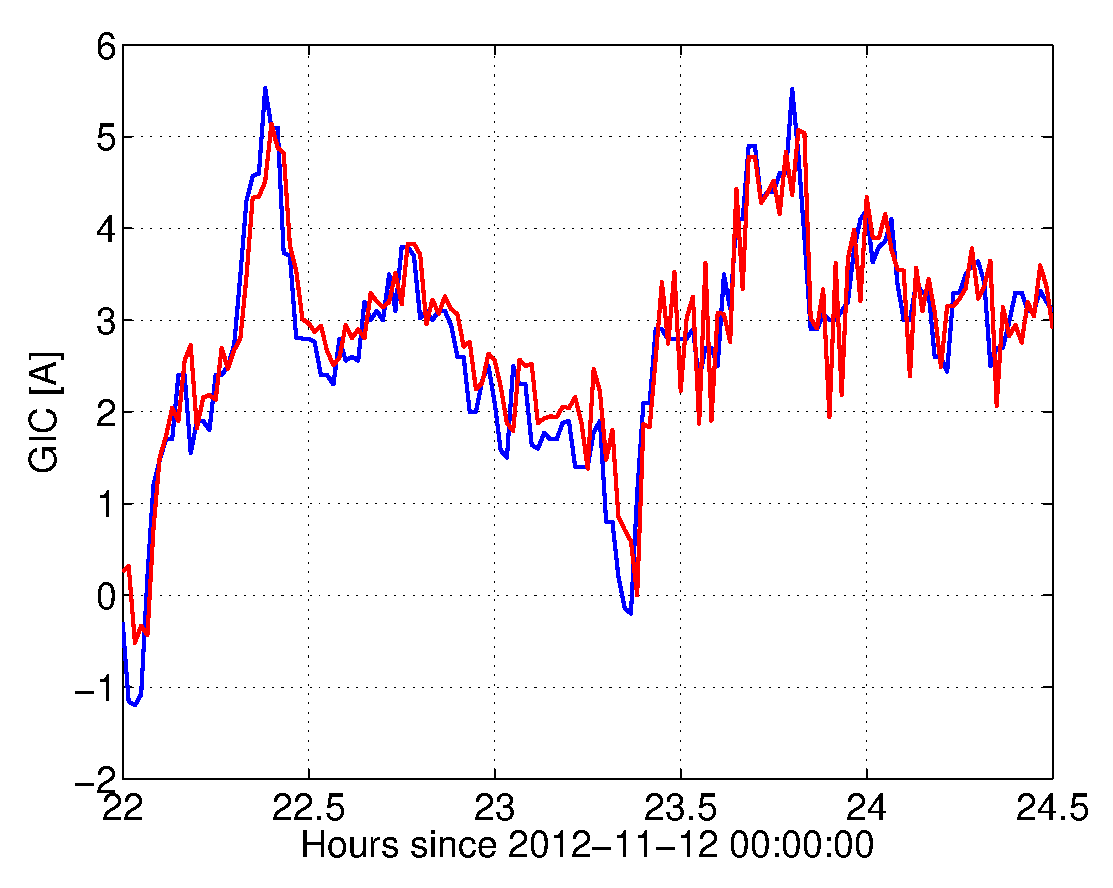
\includegraphics[scale=0.45]{{Figures/GICExample/GIC1.eps}}
	\caption{Persistence forecast; model in red}
	\label{persist}
\end{figure}

In this case, it is clear that the most recent measurement has the most weight in a forecast. For day-to-day behavior, this is acceptable as being part of the behavior of the system. For the forecasting of extreme events, however, another metric must be used that measures the ability of the model to predict events at or before their actual occurrence, while simultaneously avoiding predicting events that do not happen. One method for comparing models in this fashion is by using the Heidke Skill Score \cite{Heidke,Brier}, which is based on the quantity:
\begin{align*}
S=\frac{R-E}{T-E}
\end{align*}
where $R$ is the number of correct forecasts, $T$ is the total number of forecasts, and $E$ is the number expected to be correct by, in this case, a persistence forecast. This can be adapted to either consider a range of "correctness", or a binary threshold to be met. It may also be desired to assign a cost-weighting to success rates. If, say, it costs \$1 million to prepare a power grid for a storm, 10 false alarms to every one storm gets costly unless successfully preparing for that one storm saves \$1 billion. To do this, a measure of the utility of a forecast can be quantified \cite{WeigelDecision}:
\begin{align*}
U_F\equiv BN_H-CN_{\bar{H}}>0
\end{align*}
Where $N_H$ is the number of correct forecasts, $N_{\bar{H}}$ is the number of false alarms, $C$ is the cost of taking mitigating action, and $B$ is the benefit from correctly taking mitigating action. This method has caveats discussed in \cite{WeigelDecision}, but is a useful metric for forecast utility when costs are known, and some measure of success can be determined. 

The other major problem in forecasting is that of lead time. Being able to forecast a storm one minute in advance is generally not enough time for operators to take mitigating action.

\begin{figure}[h!]
	\centering
	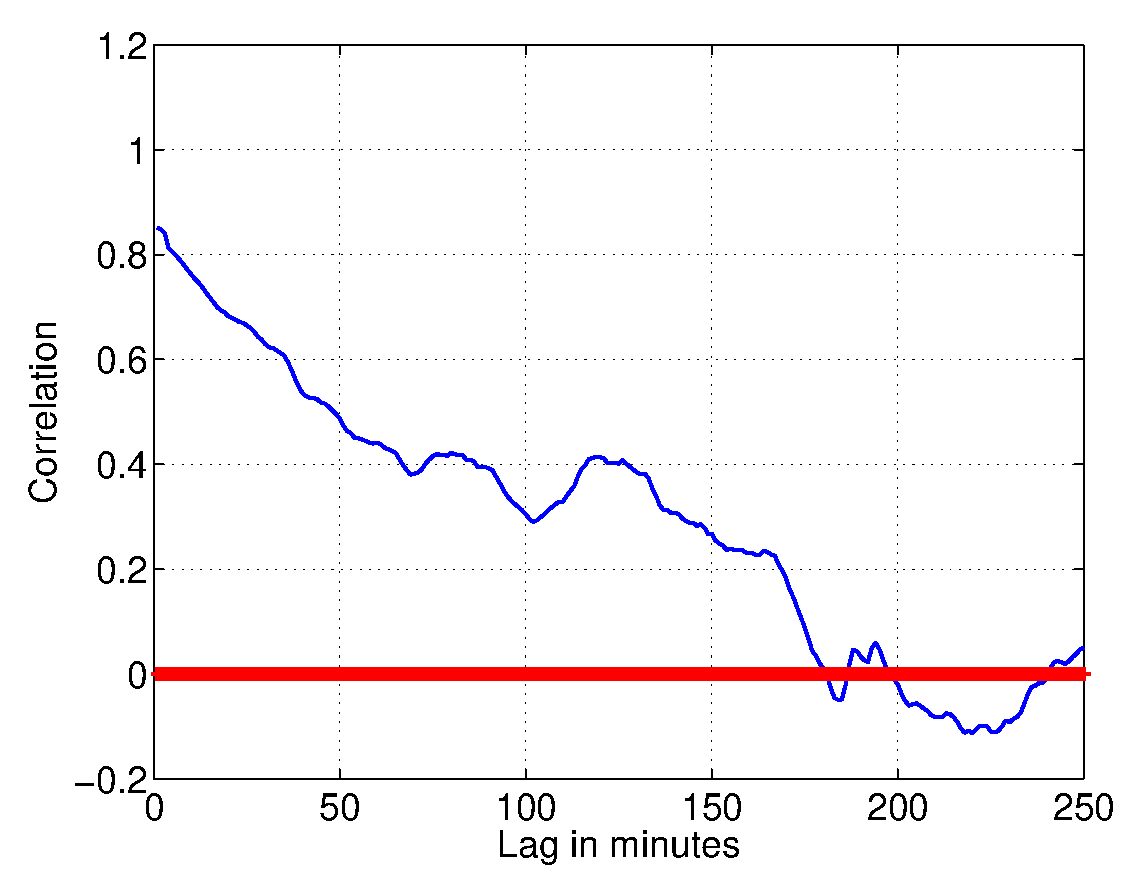
\includegraphics[scale=0.50]{{Figures/GICExample/GIClags.eps}}
	\caption{Correlation vs lags}
	\label{Lags}
\end{figure}

Figure \ref{Lags} shows a set of predictions made for autocorrelation in geomagnetically-induced currents (GIC). This metric is a measure of how much electric currents in the magnetosphere induce currents in ground-based electrical systems. The predictions were made further and further in time from the current magnetic field and GIC measurements, with decreasing accuracy as the predicted time got further from the current time. While an accurate prediction can be made one minute in advance, a prediction 3 hours in advance has almost no correlation with what actually happens. This is the main problem that this dissertation hopes to address.

\subsubsection{Mean vs Median}
The question of whether to use means or medians for analysis is based on what facets of the data are most important to the research. Since means biased towards outliers and medians biased against them, the decision rests on how much weight should be given to outliers (or extreme values) in a study. For example, when looking at long-term solar wind variables, intermittent spikes may not be relevant to the overall pattern of behavior being analyzed, but knowing that on a short time scale a certain day had a noticeable spike may be important. In the former case, using the median would likely be best, and using the mean for the latter. However, space physics often deals with skewed distributions and sparse data, leading to an uncertainty of which method is best, so both are and analyzed with their respective traits in mind.
\note Numerically specific result

\subsubsection{Effects of time averaging}
Similarly to the mean vs median question, the decision on if/how much to average the data over time will affect the resulting time series to be biased against intermittent spikes in value. The more time added to any particular average, the less impact any short-term changes will have on the final value.

\subsection{Summary}
Because linear models are simple, optimizable, and adequately model many physical systems, they're a good first choice for trying to determine the behavior of mass density in the plasmatrough. The relationships between solar wind, plasmatrough, and inner plasmasphere may also be detectable on the first order approximation by a linear model if not entirely linear in nature.


\section{Nonlinear}

\subsection{Overview}

While many nonlinear systems are approximated by a number of localized linear models for the sake of simplicity and ease of interpretation, the design and implementation of nonlinear models has become greatly simplified in recent years. Their use allows for determining nonlinear structure without pre-assuming any localization of the data, and as such were used to attempt forecasting in this dissertation. The first choice was a model based on neural networks \cite{NNARMA,ANNforecast} which approximates a non-linear system given a set of training data. The usefulness of this is apparent in a few key points: the weights of contribution of any particular variable to a system will likely be nonlinear in some fashion (e.g. a ground station's measurements will depend on sunlight heating the ionosphere which depends on latitude, time of year, and time of day), and allowing for the non-linear effects of saturation where perhaps the magnetosphere will behave differently after reaching certain levels of particle density or electric potential, rather than directly scaling regardless of limits.

Another algorithm known as Principal Component Analysis (PCA) can be used to take the large number of possible variables and define an orthogonal set of vectors that most efficiently encapsulate the variance in the data. By doing this, the number of variables needed for computing any linear or non-linear algorithm can be reduced and optimized, making predictions quicker while maintaining most of the predictive benefits of using all possible data, as well as indicating which variables contain the most information relevant to the predictions.


\subsection{Neural Networks}

\subsection{Applicability}
Nonlinear models are applicable when a system has more complexity than can be encapsulated by a linear model. Since they're usually a class of model that trains adaptive weights that can be tuned by known inputs and outputs, they're especially useful for systems where a large amount of training data are available.

\subsection{Caveats and Biases}
Nonlinear models can be susceptible to overfitting, since they inherently attempt to fit more complexity than a linear model, but can also be controlled via the number of inputs and weights used. They also may suggest more structure than might truly exist. Both of these problems are lessened by training with more data, if available. Figure \ref{NNvsLinear} shows a comparison of predicting equatorial mass density (\req) with the $F_{10.7}$ index and the disturbance storm time index (\dst). The neural net models (left)  shows much more structure than the linear models (right) despite being given the same data. Whether that structure reflects any real physical phenomenon, however, is a difficult problem to answer, and so both models are often compared to attempt to ascertain what structure may be valid. 

Sometimes, as in the top two plots of Figure \ref{NNvsLinear}, the structure seems to support the same conclusion where the nonlinear model just adds slight detail. Othertimes, as in the case of the lower two plots, the results seem discrepant. The linear model indicates increasing \req\ with increasing $B_z$ and increasing \f, while the nonlinear model shows a more nuanced structure with increased \req\ showing up with lower $B_z$ values, and at a range of \f\ values. Situations like these require further analysis to determine the true underlying structure.

\begin{figure}[h!]
	\centering
	\includegraphics[scale=0.35]{Figures/{NNDst-F107-rhoeq-GOES6}.eps}
		\includegraphics[scale=0.35]{Figures/{LinearDst-F107-rhoeq-GOES6}.eps}
			\includegraphics[scale=0.35]{Figures/{NNBz-F107-rhoeq-GOES5}.eps}
			\includegraphics[scale=0.35]{Figures/{LinearBz-F107-rhoeq-GOES5}.eps}
	\caption{Nonlinear models (left) vs linear models (right) of $\rho_{eq}$}
	\label{NNvsLinear}
\end{figure}


\subsection{Comparison to Linear Model}
Nonlinear models differ from linear models by incorporating some method for accounting for effects within a domain that are not seen across the entire domain. Though both models can be given the same inputs, and trained on the same outputs, the models themselves can fundamentally differ. Linear models are also generally simple to interpret (e.g. $y=2*x$ means for every change in $x$, $y$ changes by double that amount.) Nonlinear models, on the other hand, often have no simple interpretation and must be approached by testing for a range of parameters in the model to map out resulting outputs and make some interpretation of the underlying structure.

Nonlinear models can be compared to a linear model of the same data in order to assess the usefulness of accounting for nonlinear features. If both models result in similar correlation values, it can be said that the nonlinear model offers no extra insight into the structure of the system and the relationships therein. 

\subsection{Summary}
Nonlinear models are a useful addition to linear models by allowing for better approximations to more complex physical systems, where the entire system may not fit a linear model or may have localized dependencies. 





%% Note: appendix is now put before bibliography.
%% include the following directives if there are any appendices
\appendix
\appendixeqnumbering

%% A sample appendix
%%
%%**********************************************************************
%% Legal Notice:
%% This code is offered as-is without any warranty either
%% expressed or implied; without even the implied warranty of
%% MERCHANTABILITY or FITNESS FOR A PARTICULAR PURPOSE!
%% User assumes all risk.
%% In no event shall any contributor to this code be liable for any damages
%% or losses, including, but not limited to, incidental, consequential, or
%% any other damages, resulting from the use or misuse of any information
%% contained here.
%%**********************************************************************
%%
%% $Id: Appendix.tex,v 1.5 2006/08/24 21:12:47 Owner Exp $
%%

% N.B.: an appendix chapter starts with "appchapter" instead of "chapter"
%
% The first argument in [ ] is the title as displayed in the table of contents
% The second argument is the title as displayed here.  Use \\ as appropriate in
%   this title to get desired line breaks
\appchapter[An Appendix]{An Appendix}

This is an appendix.  Here is a numbered appendix equation:
\begin{equation}
    a^2 + b^2 = c^2.
\end{equation}


%%
%%  bibliography
%%

%% list all of the BibTeX files here for the WinEdt project (if applicable)
%GATHER{bibfile.bib}

%% any bibliography style can be used, but IEEEtran.bst is ideally suited to
%% electrical engineering references

\bibliographystyle{IEEEtran}
\bibliography{bibfile}

%%
%% curriculum vitae
%%
\cvpage

\noindent Include your \emph{curriculum vitae} here detailing your background,
education, and professional experience.
\end{document}
